\documentclass[11pt,a4paper]{article}

% -------------------------------------------------
% Packages
% -------------------------------------------------
\usepackage[utf8]{inputenc}
\usepackage[T1]{fontenc}
\usepackage{lmodern}

\usepackage{amsmath,amssymb}
\usepackage{graphicx}
\usepackage{booktabs}
\usepackage{hyperref}
\usepackage{geometry}
\usepackage{listings}
\usepackage{xcolor}
\usepackage{cite}
\usepackage{algorithm}
\usepackage{algpseudocode}

\usepackage{tikz}
\usetikzlibrary{positioning}


\geometry{margin=1in}

% -------------------------------------------------
% Listings configuration for C++
% -------------------------------------------------
\lstset{
  language=C++,
  basicstyle=\ttfamily\small,
  keywordstyle=\color{blue},
  commentstyle=\color{gray},
  stringstyle=\color{red!70!black},
  numbers=left,
  numberstyle=\tiny,
  stepnumber=1,
  numbersep=8pt,
  frame=single,
  breaklines=true,
  showstringspaces=false
}

% -------------------------------------------------
% Title Information
% -------------------------------------------------
\title{%
  \texttt{BioMesh} Algorithms and Data Structures
}

\author{
  Gautam Ghosh\\
  \small Institute for Parallel and Distributed Systems, University of Stuttgart.\\
  \small \texttt{gautam.ghosh@ipvs.uni-stuttgart.de}
}

\date{\today}

% -------------------------------------------------
% Document
% -------------------------------------------------
\begin{document}

\maketitle

% -------------------------------------------------
\section{Algorithms}

\subsection{Fiber Grid Generation}

For generating 1D fibers we need to answer 3 fundamental questions:
\begin{itemize}
    \item Where does a fiber begin ?
    \item Where does a fiber end ?
    \item What are the bounds of the muscle ?
\end{itemize}
\\
The \texttt{Seed Surface Generation} routine provides the surface on which the \texttt{Seed Points} are computed. This surface contains the Seed Points, these points mark the beginning of a fiber.\\
\\
The \texttt{Cell Classification} routine is the solution to the final 2 questions. The classification contains data about the muscle bounds. The '1' cells mark the end of a fiber. Refer to the \texttt{Algorithms} section for detailed explanation.\\
\\
The fiber generation workflow follows these steps sequentially:

\begin{itemize}
    \item \texttt{Cell Classification}
    \item \texttt{Seed Plane Generation}
    \item \texttt{Seed Point Generation}
    \item \texttt{Fiber generation}
    \item \texttt{Fiber grid generation}
\end{itemize}

\subsubsection{Description}

\begin{itemize}

\item \textbf{Cell Classification}

The first step is to identify the bounds of vector field. It represents the region within the structured grid where the fibers are allowed to flow freely.\\
    \\
    The VTK cells are classified as '0', '1', or '2' cell. The definitions are as follows:
    \begin{itemize}
        \item '0' cell : The VTK cells which do not have vectors on any corners.
        \item '1' cell : The VTK cells which have vectors on some but not all corners.
        \item '2' cell : The VTK cells which have vectors on all corners.
    \end{itemize}
    \\
    The '1' cells represent the bounds of the vector field. The fibers are allowed to flow
    freely in the '1' and '2' cells.\\
    \\
    Source files: \texttt{\textbf{biomesh\_cell\_table.hpp}}, \texttt{\textbf{biomesh\_cell\_table.cpp}}\\
    \\
    \texttt{\textbf{Algorithm:}}
\begin{algorithmic}[1]
    \Require Structured grid $G$
    \Ensure Classification label $cell\_type$ for each cell $c \in G$

    \ForAll{cells $c \in G$}
        \State $V \gets \emptyset$ \Comment{Initialize vector set for cell corners}
        \ForAll{corners $v$ of $c$}
            \State Obtain vector $\mathbf{v}$ at corner $v$
            \State $V \gets V \cup \{\mathbf{v}\}$ \Comment{Add vector to set}
        \EndFor

        \If{ $\|\mathbf{v}\| = 0 \ \forall \mathbf{v} \in V$ }
            \State $cell\_type \gets 0$ \Comment{All zero vectors}
        \ElsIf{ $\|\mathbf{v}\| \neq 0 \ \forall \mathbf{v} \in V$ }
            \State $cell\_type \gets 2$ \Comment{All non-zero vectors}
        \Else
            \State $cell\_type \gets 1$ \Comment{Mixed zero and non-zero vectors}
        \EndIf
    \EndFor
\end{algorithmic}

\item \textbf{Seed Plane Generation}

    The second step is identify the beginning of the fibers. The \texttt{Seed Plane} splits the vector field in two parts. Naturally, the \texttt{Seed Plane} intersects the structured grid cells. The plane-cell intersection is a surface triangulation.\\
    The seed points will be computed on this surface.\\
    
    \\
    Source files: \texttt{\textbf{biomesh\_seed\_plane.hpp}}, \texttt{\textbf{biomesh\_seed\_plane.cpp}}\\
    \\
    \texttt{\textbf{Algorithm:}}
\begin{algorithmic}[1]
    \Require Structured grid $G$, cell classification C
    \Ensure Triangle set $T$ containing valid intersections

    \State $T \gets \emptyset$ \Comment{Initialize triangle set}
    \State Construct plane $P$
    \State $S \gets P \cap G$ \Comment{Surface triangulation S from intersecting P with G}

    \ForAll{triangles $t \in S$}
        \State $c \gets \text{centroid}(t)$
        \State $cell \gets \text{cell containing } c$
        \If{$c \notin G$} 
            \State \text Skip $t$ 
        \EndIf
        \If{$C(cell) = 2$} 
            \State $T \gets T \cup \{t\}$ \Comment{Add triangle if cell type indicates valid region}
        \EndIf
    \EndFor
\end{algorithmic}\\
\vspace{5em}
\item \textbf{Seed Point Generation}

    The thrid step is compute the seed points. These points are the initial conditions for the numeric integration scheme. The Random Sampling technique is used to generate the points.\\
    First, the center of the triangles are computed. Then the triangles whose centers are within the bounds of the '2' cells are checked. If their centers are within the '2' cell bounds then the center is flagged as a seed point.\\
    \\
    Source files: \texttt{\textbf{biomesh\_seeder.hpp}}, \texttt{\textbf{biomesh\_seeder.cpp}}\\
    \\
    \texttt{\textbf{Algorithm:}}
\begin{algorithmic}[1]
    \Require seed plane $P$, seed count $C$
    \Ensure Seed vertex set $S$

    \State $S \gets \emptyset$ \Comment{Initialize set of seed vertices}
    \State $A \gets \emptyset$ \Comment{Cumulative area array}
    \State $TotalArea \gets 0$

    \ForAll{triangles $t \in P$}
        \State $TotalArea \gets TotalArea + \text{Area}(t)$
        \State $A \gets A \cup \{TotalArea\}$
    \EndFor

    \State Initialize random number generator $R$

    \For{$i = 0$ \textbf{to} $C-1$}
        \State $r \gets$ random value from $R$ scaled by $TotalArea$
        \State Find triangle $t \in P$ corresponding to index $r$ in $A$
        
        \State $u \gets$ random value from $R$  \Comment{Barycentric weights}
        \State $v \gets$ random value from $R$
        \State $w \gets 1 - u - v$
        
        \State Let $p_0, p_1, p_2$ be vertices of triangle $t$
        \State $seed \gets w \cdot p_0 + u \cdot p_1 + v \cdot p_2$
        
        \State $S \gets S \cup \{seed\}$ \Comment{Add generated seed to set}
    \EndFor
\end{algorithmic}

\item \textbf{Fiber Generation}

    The fourth step is to execute the \texttt{Runge-Kutta4} scheme to trace the fibers. \\
    \\
    Source files: \texttt{\textbf{biomesh\_fiber3d.hpp}}, \texttt{\textbf{biomesh\_fiber3d.cpp}}\\
    \\
    \texttt{\textbf{Algorithm:}}
\begin{algorithmic}[1]
    \Require Structured grid $G$, cell classification $C$, configuration parameters $T$, direction $D$
    \Ensure Fiber $f$ generated from seed vertex $s$

    \State $t_{\text{start}} \gets 0$
    \State $\Delta t \gets vertex\_width(T)$
    \State $vc \gets vertex\_count(T)$
    \State $s \gets$ seed vertex
    \State Initialize Runge--Kutta 4 integrator $I$

    \If{$ strategy(T) = \text{static}$}
        \State $\text{adaptivity} \gets \text{false}$
    \ElsIf{$ strategy(T) = \text{adaptive}$}
        \State $\text{adaptivity} \gets \text{true}$
    \EndIf

    \State $N_{\text{adaptive}} = 0$
    \State $N_{\text{adaptive}}^{\max} \gets \text{adaptive\_steps\_max}(T)$

    \State $cid \gets \mathrm{Index}\!\left(
    \left\{ c \in G \mid s \in c \right\}
\right)$

     \While{$C(cid) = 1 \lor C(cid) = 2$}

        \If{$\neg \text{adaptivity} \;\lor\; 
            (\text{adaptivity} \land N_{\text{adaptive}}^{\max} \text{ reached})$}

            \State $v_{curr} \gets s$
            \If{ $v_{curr} \neq \text{last}(f)$}
                \State $f \gets f \cup \{v_{curr}\}$ \Comment{Append vertex to fiber}
            \EndIf
        \EndIf

        \State $cid \gets \mathrm{Index}\!\left(
    \left\{ c \in G \mid v_{curr} \in c \right\}
\right)$
        \State $v_{previous} \gets v_{curr}$
        \State $v_{curr} \gets I(G, v)$ \Comment{Advance one integration step}

        \If{$v_{curr} \neq v_{previous}$}
            \State $v_{diff} \gets v_{new} - v_{previous}$
            \If{\text{$D \gets 1$}}
                \State $v_{diff} \gets -v_{diff}$
            \EndIf
        \EndIf

        \If{$C(i) = 0$}
            \If{$\text{adaptivity}$ }
                \If{$N_{\text{adaptive}}^{\max} = N_{\text{adaptive}}$}
                    \State \textbf{break}
                \Else
                    \State $\Delta t \gets \frac{\Delta t}{2}$ \Comment{Reduce step size}
                    \State $N_{\text{adaptive}} \gets N_{\text{adaptive}} + 1$
                \EndIf
            \Else
                \State \textbf{break}
            \EndIf
        \EndIf

        \State v_{\text{curr}} \gets v_{previous} + \frac{v_{diff}}{\|v_{diff}\|}\\
        \State $t_{\text{start}} \gets t_{\text{start}} + \Delta t$

    \EndWhile
\end{algorithmic}
\item \textbf{Fiber Grid Generation}

    The final step is to execute the fiber generation routine for every \texttt{Seed Point} to generate the \texttt{Fiber Grid}.This is done in two steps ( Forward and backward ). For every seed point, the fiber is computed in the direction of the vector field flow (Forward) and then in the opposite direction of vector field flow (backward).\\
    \\
    Source files: \texttt{\textbf{biomesh\_fiber\_grid.hpp}}, \texttt{\textbf{biomesh\_fiber\_grid.tpp}}\\
    \\
    \texttt{\textbf{Algorithm:}}
\begin{algorithmic}[1]
    \Require Structured grid $G$, seed set $S$
    \Ensure Fiber grid $F$

    \State $F \gets \emptyset$ \Comment{Initialize fiber grid}

    \ForAll{seeds $s \in S$}
        \State $f \gets \text{generate\_fiber}(s, G, backward)$
        \State $f \gets \text{reverse($f$)}$      \Comment{reverse the order for vertices}
        \State $f \gets \text{generate\_fiber}(s, G, forward)$
        \State $F \gets F \cup \{f\}$ \Comment{Insert generated fiber into grid}
    \EndFor
\end{algorithmic}

\section{Data Structures}

\subsection{\texttt{fiber}:}
A single fiber is represented as a contiguous array of vertices.\\
\\
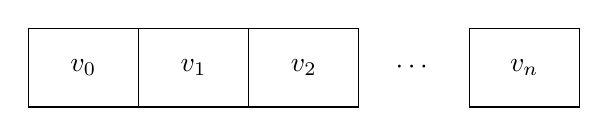
\begin{tikzpicture}
  % First elements
  \foreach \i/\val in {0/v_0,1/v_1,2/v_2} {
    \draw (1.4*\i,0) rectangle ++(1.4,1);
    \node at (1.4*\i+0.7,0.5) {$\val$};
    %\node[below] at (1.4*\i+0.7,0) {\texttt{a[\i]}};
  }

  % Ellipsis
  \node at (1.4*3+0.7,0.5) {$\cdots$};

  % Last element
  \draw (1.4*4,0) rectangle ++(1.4,1);
  \node at (1.4*4+0.7,0.5) {$v_n$};
  %\node[below] at (1.4*4+0.7,0) {\texttt{a[n-1]}};
\end{tikzpicture}

\subsection{\texttt{fiber\_grid}:}
All fibers are stored using an \texttt{'array-of-arrays'} data structure.\\
\\
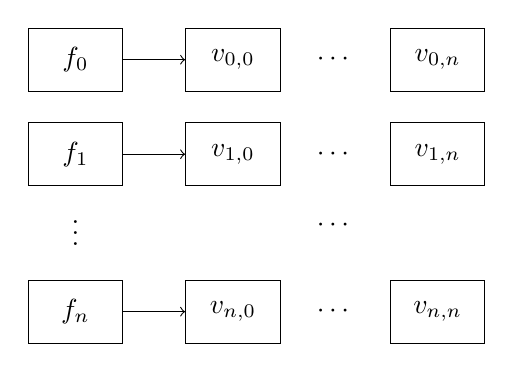
\begin{tikzpicture}[
  cell/.style={draw, minimum width=1.2cm, minimum height=0.8cm},
  main/.style={cell},
  sub/.style={cell}
]

% Main vertical array
\node[main] (f0) at (0,0) {$f_0$};
\node[main] (f1) at (0,-1.2) {$f_1$};

\node at (0,-2.1) {$\vdots$};

\node[main] (fn) at (0,-3.2) {$f_n$};

% Sub-array for f0
\node[sub] (f00) at (2,0) {$v_{0,0}$};
\node at (3.3,0) {$\cdots$};
\node[sub] (f0k) at (4.6,0) {$v_{0,n}$};
\draw[->] (f0.east) -- (f00.west);

% Sub-array for f1
\node[sub] (f10) at (2,-1.2) {$v_{1,0}$};
\node at (3.3,-1.2) {$\cdots$};
\node[sub] (f1k) at (4.6,-1.2) {$v_{1,n}$};
\draw[->] (f1.east) -- (f10.west);

% Ellipsis for intermediate rows
\node at (3.3,-2.1) {$\cdots$};

% Sub-array for fn
\node[sub] (fn0) at (2,-3.2) {$v_{n,0}$};
\node at (3.3,-3.2) {$\cdots$};
\node[sub] (fnk) at (4.6,-3.2) {$v_{n,n}$};
\draw[->] (fn.east) -- (fn0.west);

\end{tikzpicture}

\end{document}